\chapter{User-Centered Design}
\label{chapter:stakeholders_personas} 
In software development and \ac{ux} design, understanding the diverse array of individuals who interact with or are affected by a system is imperative, as this understanding forms the cornerstone to create solutions that not only function well but also are tailored and resonate deeply with their intended users. 
\\ 
This chapter undergoes a comprehensive exploration of stakeholders and personas, exploring into their motivations and the scenarios in which they operate. By identifying key stakeholders and developing detailed personas, we aim to create an accurate portrayal of our user base. This approach allows the development team to empathize with target audiences needs, anticipate their challenges, and design solutions that truly address their pain points. 
\\ 

\section{Stakeholders}
\label{section:stakeholders} 
The following list presents the key stakeholders (and individuals or groups who have high interest in the project’s outcome) identified for the \ac{splash} system: 

\begin{itemize}
    \item \textbf{Primary Stakeholders - Lifeguards:}
    \begin{itemize}
        \item Play a critical role in ensuring beach safety.
        \item Primary users of the \ac{splash} system.
        \item Benefit from tools for real-time monitoring, efficient incident prevention and management, and proactive hazard identification.
        \item System designed to support and enhance their performance.
    \end{itemize}

    \item \textbf{Secondary Stakeholders - Beachgoers:} 
    \begin{itemize}
        \item Interact with the web application.
        \item View and report beach hazards, providing valuable information for lifeguards.
        \item Access information on lifeguard locations.
        \item View beach-related information such as weather conditions.
    \end{itemize}

    \item \textbf{Secondary Stakeholders - Beach Business Owners:} 
    \begin{itemize}
        \item Interact with the web application as beachgoers.
        \item Can increase their business clientele and profits by accessing premium features through a paid account, which enables them to list their business information, prices, location, and more.
        \item Provide an initial monetization avenue for the system.
    \end{itemize}
\end{itemize}

\section{Personas, Motivations \& User Scenarios}
\label{section:personas}

The main personas are described in the following list:

\begin{itemize}
    \item \textbf{Lifeguard Supervisor}
    \item \textbf{Regular Lifeguard}
    \item \textbf{Beachgoer}
    \item \textbf{Business owner}
\end{itemize}

\subsection{Lifeguard Supervisor}
\subsubsection{\textbf{Biography}}
Miguel is a 34 year old lifeguard, born on October 14, 1990, in Funchal (Madeira), and raised in Cascais, where he was always immersed in beach life and water activities. Miguel has always held a deep affection for the beaches and sea of his home-town and later embarked on various journeys along Portugal’s coastline to experience the country's diverse beaches and tides. Thanks to his lifelong connection to the sea, Miguel knew he wanted to work close to it. He took a degree in Physical Education and Sports while also completing certifications as a lifeguard and teacher. He began working as a lifeguard during beach seasons, and outside of these periods, he worked in gyms and fitness academies, teaching swimming and functional training.

Miguel’s first experience as a lifeguard was both enriching and challenging. His training provided him with all the tools he needed for the job, but theoretical knowledge couldn’t replace the practical skills acquired on the field. He initially struggled with maintaining near-constant focus on beach-goers and often found himself frustrated by swimmers choosing less visible spots. Thankfully, his more experienced colleague supported him every step of the way. Today, Miguel considers the most important lesson from those early days to be the value of having a mentor during the learning process. In the years that followed, Miguel worked as a Swimming Instructor and Swimming Team Coach, roles that complemented and were complemented by his work as a lifeguard. At 28, he became a Physical Education Teacher. Here, he directly experienced some of the frustrations of parents he had often observed at the beach, trying their best to supervise children or manage certain activities.

Now considered a veteran within the lifeguard community, Miguel takes on the role of mentor for novices and aspiring lifeguards who choose to embrace the challenge. He recognizes in their mistakes and frustrations the same ones he experienced many years ago. But while some things remain unchanged, many others have evolved. Technology has advanced exponentially since his childhood. Mobile phones have become smartphones, the internet is now wirelessly accessible, and weather forecasts have become more accurate and available in real-time. Miguel also sees a stronger attachment to technology among the newer generations and a greater disconnect from the environment. He believes that with the right approach, technology can be used to complement human limitations.

\subsubsection{\textbf{Motivation}}
Miguel wants to improve the management of lifeguard teams. He seeks a broader and more integrated view of the beach environment, as well as tools for signalling hazardous situations.
\subsubsection{\textbf{Mega Scenario: ``A Summer Day: Management and Surveillance''}}
\subsubsection{\textbf{Scenario 1:} Miguel Logs in to Monitor the Beach and Approves a New Lifeguard Registration}
Miguel starts his day by checking the beach monitoring system. He accesses the required URL, clicks on Login, and enters his credentials before clicking ``Submit.'' He then views the camera activity and hazard zones on the interactive map. While observing the beach in real-time, he ensures that the busiest areas are monitored and adjusts the interactive map to assign teams to specific monitoring zones by clicking on the location of each lifeguard post and allocating team members based on their schedules via the ``Schedule'' tab. 

A few minutes later, he receives information about the registration of a new lifeguard. Miguel accesses the ``Team Management'' section and confirms the registration by clicking the ``Accept'' button, allowing the new team member to begin their duties.

\subsubsection{\textbf{Scenario 2:} Miguel Receives a Request to Analyze a Hazard Zone for Weever Fish Stings and Sends a Lifeguard to Investigate}
Miguel receives an alert on his interactive map. He clicks on the red circle with the ``eye'' icon and sees that a beachgoer has requested an analysis of a hazard zone due to ``Weever Fish Sting.'' Miguel quickly clicks the ``Send Lifeguard'' button and selects the nearest lifeguard to investigate. Moments later, the hazard zone is confirmed by his colleague. Miguel then adjusts the hazard zone settings, draws the specific area on the screen with his finger, and clicks ``Issue Alert,'' sending a visual notification (map drawing) to all beachgoers with system access, indicating the danger zone. He feels satisfied knowing the information is quickly disseminated, ensuring safety.

\subsubsection{\textbf{Scenario 3:} Miguel Receives an Emergency Notification About a Lost Child}
An alert notification arrives on his system: ``Bracelet associated with a child is emitting an alert signal.'' Miguel immediately clicks the ``Respond'' button and, with the guardian's automatic authorization, checks the GPS location of the child. He then clicks the ``Send Lifeguard'' button, assigning lifeguard Joana Costa, who is the closest to the child's location, to the emergency. Joana quickly proceeds to handle the situation.

\subsubsection{\textbf{Scenario 4:} Miguel Observes and Coordinates the Rescue of a Swimmer Using a Drone and Detection Cameras}
Through the camera mounted at the lifeguard post, Miguel notices that a swimmer, Maria Fernandes, has crossed the safety limit and appears to be in trouble in the water. Based on his experience, he quickly deduces that Maria is suffering from a cramp and is in a location where she cannot touch the bottom. Miguel immediately clicks the ``Pre-Drowning'' button and marks the approximate location on the map, alerting the nearest lifeguard. 

He then clicks the ``Send Drone'' button, puts on the VR goggles, and takes control of Rescue Drone No. 1, which emits its GPS location to the field lifeguard system. Moments later, the drone reaches Maria's location, and Miguel uses the drone's speaker to communicate: 
``Stay calm. I’m dropping a rescue buoy. Hold on and stretch your leg to relieve the cramp. Help is on the way.'' He commands the drone to release the rescue buoy. Shortly after, lifeguard Joana Costa arrives to assist Maria.

After resolving the issue, Miguel accesses the interactive map in the application, draws a red circle around the dangerous area, and marks it as ``Rip Current,'' sending a visual notification (drawing) to beachgoers and colleagues about the zone.

\subsubsection{\textbf{Scenario 5:} Miguel Corrects Errors by Analysing Weather Conditions, Updates the Flag Status, and Accesses the Beach History and Metrics}
Miguel accesses his interactive map and reviews the ``Weather Conditions'' tab, which shows favourable conditions for beach activities (Temperature: 35ºC, Waves: 0.5 meters, Wind: 1 km/h, etc.). He verifies that the flagged status is correct (green) but notices that the system indicates the wrong flag. He clicks on the yellow flag icon at the respective post and changes it to ``Green.'' 

Later, he accesses the ``History and Metrics'' tab. This section provides a complete history and metrics of the beach (e.g., Problematic Areas, Average Number of Incidents per Month/Year). Using this data, Miguel begins to design future safety strategies based on the insights from this section.

\subsubsection{\textbf{End of the Mega Scenario}}
At the end of the day, Miguel reflects on how technology has improved communication and the efficiency of his team.


\subsection{Regular Lifeguard}
\subsubsection{\textbf{Biography}}
Joana Costa is a 19 year old lifeguard, born on April 26,2005 , in Portimão. From an early age, her connection to the sea shaped her passion for the beach and aquatic environments. At just two years old, she began swimming and, over the years, developed into a talented competitive athlete.

In 2023, Joana decided to follow her passion and enrolled in the Bachelor’s program in Sports Science at the University of Coimbra. However, after a few months in the course, her parents realized they couldn’t financially support her studies beyond the first year due to the rising cost of living. Determined not to give up on her goals, Joana sought a solution and enrolled in the Lifeguard Training Course at EFNSP.

With her experience as an athlete and her deep knowledge of the aquatic environment, Joana easily passed both the physical and theoretical tests, completing the course in January 2024. By late May, she was preparing to begin her first summer season as a lifeguard. Accustomed to the calm, warm waters of the Algarve, Joana was eager to face new challenges on the beaches of the central region.

However, her first day on the job brought an unexpected twist. What started as a calm, sunny afternoon quickly changed with the arrival of a dense fog from the north, drastically reducing visibility. Concerned about the large number of swimmers in the water, Joana remained vigilant.

Suddenly, a man approached her, visibly distressed, reporting that his 13-year-old son, who had been bodyboarding, was missing. In a mix of adrenaline and focus, Joana used her binoculars to try to locate the boy, but the dense fog made it impossible to spot him. Without hesitation, she grabbed her board and entered the water to search for the boy. After 15 minutes of searching with no success, she reported the disappearance to the maritime police.

Fortunately, the rescue was successful, and the boy was found being carried by a current, with no serious injuries. Despite the positive outcome, the incident left Joana emotionally shaken. The feeling of helplessness for not being able to act faster stayed with her, challenging her to become even more vigilant and prepared for future emergencies.

\subsubsection{\textbf{Motivation}}
Joana would like to have a broader view of the beach she monitors and better communication with her colleagues.

\subsubsection{\textbf{Mega Scenario: ``A Day of Action for Joana''}}
\subsubsection{\textbf{Scenario 1:} Joana Arrives at an Unknown Beach and Logs in as a Lifeguard to Start her Shift}
Joana arrives at a new beach, excited for her first day as a lifeguard. At the entrance, she notices a QR code and decides to scan it. Joana creates an account (Sign in) and logs in. The tablet provides information about the beach, including the presence of dangerous currents and the location of other lifeguards. Two minutes later, she receives confirmation that her account has been approved by the supervising lifeguard, ``Miguel Soares,'' along with details about her schedule, team, and assigned station. This information boosts her confidence, knowing she can rely on her team's support.
\subsubsection{\textbf{Scenario 2:} Joana Receives an Emergency Alert ``Lost Child''}
While monitoring the beach from her chair, Joana receives a notification on her device: ``ALERT: Swimmer in difficulty.'' She quickly heads to the area indicated on the interactive map and encounters a worried father, Ricardo, who is trying to locate his son who has drifted too far. Joana uses a GPS bracelet to help Ricardo determine the child's location. Following the tablet's instructions, Joana quickly finds the child playing with other kids. Relieved, she brings the child back to the safe area where Ricardo is anxiously waiting. Grateful for her swift action and the use of technology that facilitated locating his son, Ricardo thanks Joana deeply. Joana then logs into her tablet and marks the situation as ``Successfully Resolved.''
\subsubsection{\textbf{Scenario 3:} Joana Is Notified to Analyse a Potential Danger Zone on the Sand}
During her shift, Joana receives an alert on her device: ``ALERT: Danger, Debris on the Sand,'' reported by a beachgoer. She quickly moves to the indicated location, where she finds broken glass, confirming the alert's accuracy. Joana physically cordons off the dangerous area and uses her tablet to alert her supervisor, Miguel, enabling him to contact the appropriate services to clean the site.
\subsubsection{\textbf{Scenario 4:} Joana Is Alerted to an Emergency and Rescues a Swimmer in Pre-Drowning}
During her shift, Joana notices a drone flying over the beach. Miguel, who is at the command post, informs her via tablet about a situation where a swimmer is drifting into open water. Using the tablet, Joana quickly confirms the swimmer's location and heads into the water. Upon entering, she spots the swimmer, Maria, in distress. Following Miguel's instructions, she uses a rescue buoy dropped by the drone to successfully save Maria.
\subsubsection{\textbf{Scenario 5:} Joana Requests a Schedule Change and Performs Shift Handover}
As her shift comes to an end, Joana is notified via tablet that she is about to be relieved by her colleague, ``Eduardo Monteiro,'' who will meet her at her station. Joana reviews her schedule and notices a conflict for the following Thursday due to a medical appointment. She clicks on the ``Lifeguard Hub'' button, selects ``My Schedule,'' and accesses the ``Calendar'' option. She then clicks on ``Request Change,'' providing the reason for the request. Next, she selects ``Shift Handover,'' where she inputs relevant details about her shift for her replacement.
\subsubsection{\textbf{End of the Mega Scenario}}
After an intense workday, Joana reflects on the importance of technology for performing rescues and fostering collaboration among lifeguards. She realizes that, even as a newcomer to the profession, she can make a significant difference with the right support.


\subsection{Business owner}
\subsubsection{ \textbf{Biography}}
Ricardo, a 40 year old beach bar owner and occasional vendor of American waffles, lives in Vila Nova de Gaia and inherited the business from his father, which is why he didn’t pursue higher education. He is married to the woman he met in his youth, and together they have two children, aged 10 and 7. One of his favourite hobbies is going to the beach with his family to enjoy quality time together.

One summer day, Ricardo went to the beach with his family, but upon arrival, he discovered that the beach was not supervised. He became worried about his children's safety since he didn’t know how to identify the most dangerous areas and had no way of predicting this situation before leaving home.

On another occasion, Ricardo took his children alone to a supervised beach, but it was very crowded, making it difficult for him to watch over both kids at the same time. This caused him more concern and limited his enjoyment of the outing.
\subsubsection{\textbf{Motivation}}
Ricardo would like to have a way to receive information about the beach he is visiting and an easier way to monitor his children while they are at the beach.

\subsubsection{\textbf{Mega Scenario: ``A Summer Day in Ricardo's Life''}}
On a sunny morning, Ricardo, a 40-year-old father, decides to enjoy his day off with his wife and two children, aged 10 and 7. Excited, the family prepares their beach essentials, applying sunscreen and packing snacks and sand toys into a bag. After a short 20-minute car ride, they arrive at their favourite beach, eager for a relaxing day.

\subsubsection{\textbf{Scenario 1:} Ricardo Visits an Unsupervised Beach and Uses the App to Get Beach Information}
Upon arriving at the beach, Ricardo notices something unsettling: the beach is not supervised by lifeguards that day. As a protective father, he quickly feels the responsibility to ensure his children’s safety. With his heart racing and worried about currents and potential hazards, he begins to look for solutions.

Noticing a QR code posted at the beach entrance, Ricardo scans it with his phone. The code redirects him to a website with detailed information about the beach conditions. The technology provides him with a sense of relief. On the site, he finds a map indicating areas with weaker currents and the location of submerged rocks — crucial information for ensuring his family’s safety. The site also offers safety tips for dealing with unsupervised beaches, which reassures Ricardo.

Armed with this knowledge, Ricardo takes a deep breath and guides his family to a designated safe area. There, they can finally relax and enjoy their day without the constant feeling of imminent danger. Still attentive, Ricardo feels more at ease knowing he is well-informed.

\subsubsection{\textbf{Scenario 2:} Ricardo Visits a Supervised Beach Offering GPS Bracelets}
Later, after lunch, Ricardo’s wife returns to work, and he decides to head back to the beach with his two children. This time, the beach is supervised, and upon advice from another beachgoer, Maria Fernandes, he scans the QR code again and discovers something new. The site informs him that the lifeguard post offers a GPS bracelet system to monitor children. This immediately captures his attention, as being alone with two active children makes him feel the need for additional safety measures.

Ricardo approaches the lifeguard post, where he meets Joana, a young lifeguard who assists him. She explains that the GPS bracelets allow real-time monitoring of children’s locations and send alerts if they stray beyond a predefined radius. Impressed, Ricardo decides to rent three bracelets: one for himself and two for his children.

Throughout the afternoon, Ricardo relaxes while watching his children play, with the added peace of mind that he will be immediately notified if something happens. Whenever one of the children tries to leave the safe area, Ricardo’s bracelet vibrates softly, alerting him to call his children back.

\subsubsection{\textbf{Scenario 3:} One of Ricardo’s Children Disappears on the Beach with the GPS Bracelet}
Near the end of the afternoon, as Ricardo relaxes, he feels a vibration on his wrist. One of his children has wandered beyond the safe zone set by the GPS bracelet. Ricardo’s heart races. He looks around, but the crowded beach makes it difficult to locate his child immediately. Panic begins to set in.

Realizing his child is missing, Ricardo rushes to Joana, the lifeguard. He quickly explains the situation, and Joana, calm and experienced, asks if the child is wearing one of the GPS bracelets. Ricardo confirms, and Joana uses a tablet equipped with a compatible reader. By linking Ricardo’s bracelet to the system, Joana quickly locates the exact position of all family members and identifies Ricardo’s child.

The tablet shows the child is further away, playing with other kids. The tension in Ricardo’s chest eases as Joana accompanies him to where his child is, safe and sound. Relieved, Ricardo thanks her for her help and reflects on how this technology made a huge difference during such a stressful moment.

\subsubsection{\textbf{Scenario 4:} Ricardo Upgrades His Account to Premium}
Back at his beach bar, Ricardo accesses the application and notices a new button labeled ``Promote Beach Business.'' Curious, he clicks on it and learns that, for a modest monthly fee, he can upgrade his user account to a premium account. This allows him to promote his business by displaying information such as ``Profile Picture,'' ``Business Name,'' ``Business Type,'' ``GPS Location,'' ``Description,'' ``Products,'' and ``Prices.''

Ricardo clicks the ``Get Premium Account'' button and is redirected to the plan selection and payment page. After selecting a plan and payment method, he enters the necessary credentials and completes the payment, obtaining a premium account. He then clicks on the new ``Manage Business'' button and accesses the business management menu. Ricardo updates his profile by editing the relevant fields such as ``Profile Picture,'' ``Business Name,'' ``Business Type,'' and ``Description.'' After submitting the changes, he returns to the business management menu and begins adding his products, prices, and promotions.

\subsubsection{\textbf{End of the Day}}
As the sun sets, Ricardo and his children return home, tired but happy. Reflecting on the day, he realizes how small technologies, such as the simple QR code at the beach entrance and the GPS bracelets, made a big difference. These innovations not only ensured his children’s safety but also gave him peace of mind that would have been hard to achieve without them. More than just a fun day, it was a day of trust and security.

\subsection{Beachgoer}
\subsubsection{ \textbf{Biography}}
Maria is an experienced nurse, 49 years old, born on February 7, 1975, in Braga. She grew up in Vila do Conde with her sister Regina, where they spent summers at the local beach, making Maria a regular beachgoer and nurturing her special affection for the sea.

One day, Maria was swimming at Armação de Pêra beach, which she had never visited before. Suddenly, she realized she was drifting far from the shore, and no matter how hard she tried to swim back, she was being pulled further out to sea. To make matters worse, she began to experience a cramp in her left leg, severely hindering her ability to move. Fortunately, Maria managed to catch the attention of a lifeguard who reached her several meters from the shore. He handed her a rescue buoy, stretched her leg to treat the cramp, and advised her to swim perpendicular to the shoreline to escape the rip current. Exhausted and shaken, Maria made it back to the sand. She hadn’t known about the rip current in that area, which left her feeling apprehensive. She decided not to swim anymore that day and opted instead to take a walk along the water’s edge.

During her walk, Maria ventured beyond the lighthouse, but upon her return, she realized the area was flooded due to the high tide. She had to use a staircase several meters away to access the promenade and return to safety. This experience frustrated her, as she had to walk much further to find an accessible staircase, leaving her very tired.

Maria earned her nursing degree from the Escola Superior de Enfermagem de Coimbra. With 25 years of professional experience, she specialized in critical care nursing and has worked in an Intensive Care Unit, treating numerous cases of patients in post-drowning situations.

Her personal and professional experiences have shaped her attitude toward beach safety. Maria prefers to visit beaches supervised by lifeguards, understanding the potential dangers of the sea. However, she is aware that it’s not always easy to determine whether a beach is supervised or to identify hazardous areas within the same beach.

At 49 years old, Maria reflects on how the beach can be a relaxing activity but also potentially dangerous without adequate rescue resources or supervision.
\subsubsection{\textbf{Motivation}}
Maria would like to have a technological solution that provides information about hazardous areas and the safety of the beaches she may visit.
\subsubsection{\textbf{Mega Scenario: ``A Day at Praia da Rocha''}}
It was a sunny day at Praia da Rocha, one of the most popular beaches in the Algarve. Maria de Lurdes da Silva Fernandes, a 49-year-old nurse, was about to experience a day at the beach that would change her perspective on beach safety, thanks to innovative technologies.

\subsubsection{\textbf{Scenario 1:} Maria Uses the App to Learn More About the Beach}
Upon arriving at Praia da Rocha, Maria notices a QR code on a sign at the entrance that reads: “Access our app for more information about this beach.” Curious, she scans the code with her smartphone and is redirected to an app displaying an interactive map of the beach. The map provides relevant information such as submerged rocks, areas with strong currents and rip currents, the locations of lifeguards, and more, all clearly marked.

In the top corner, she sees an icon indicating the current flag status (“green”), confirming that the beach is supervised, along with the UV radiation level.

\subsubsection{\textbf{Scenario 2:} Maria Pairs Her Smartband with the App}
After setting up her beach umbrella and towel, Maria opens the app to pair her waterproof Smartband. She clicks on the menu icon in the top-left corner (three horizontal lines) and selects the ``Pairing'' option from the dropdown menu. Then, she clicks ``Scan QR Code'' and scans the QR code on her Smartband. Now, she can receive alerts while swimming.

\subsubsection{\textbf{Scenario 3:} Maria Receives Alerts on Her Smartband}
Eager to enjoy the water, Maria enters the sea. After a few minutes of swimming, her Smartband vibrates, displaying a notification: “Caution: Strong currents 5 meters ahead.” The alert is accompanied by a visual warning on the band’s display. Feeling prepared, Maria changes direction and swims away from the dangerous area.

\subsubsection{\textbf{Scenario 4:} Maria Experiences Difficulties and Receives Help from a Drone}
Unfortunately, while enjoying the water, Maria experiences a cramp in her leg. She struggles against the waves, trying to return to shore, but the pain is severe. Suddenly, a drone flies overhead. Through its speaker, she hears the calm voice of veteran lifeguard Miguel Soares from the command post: “Stay calm. I’m dropping a buoy. Hold on and stretch your leg to relieve the cramp. Help is on the way.” Following his instructions, Maria takes deep breaths and swims in the suggested direction. Within minutes, she sees Joana Costa, the novice lifeguard, approaching to assist her.

\subsubsection{\textbf{Scenario 5:} Maria Searches for Beach Bars Using the App}
Feeling hungry, Maria opens the app to search for places to eat on the beach. On the main screen (the beach map), she notices two bars marked on the interactive map. Clicking on one of the locations redirects her to a page displaying the bar's name, menu, and prices.

\subsubsection{\textbf{Scenario 6:} Maria Receives a Notification About a High Tide Area}
After eating, Maria decides to take a walk along the shore. While enjoying the view, her smartphone vibrates with a notification: “Caution! The area ahead is prone to flooding during high tide. In 50 meters, you will enter an unsupervised area.” Grateful for the warning, she decides to return to a safer area, avoiding any risk.

\subsubsection{\textbf{Scenario 7:} Maria Reports Hazardous Glass on the Sand}
While walking along the beach, Maria notices broken glass on the sand. She takes out her smartphone, opens the app, and clicks on her current location on the interactive map to access reporting options. Selecting “Report Issue,” she chooses “Hazardous Waste” and then “Glass,” finally clicking “Submit.” A confirmation pop-up appears: “Issue Reported.” Satisfied, Maria continues her walk, taking extra care to avoid stepping on any glass.

\subsubsection{\textbf{Scenario 8:} Maria Assists an Injured Beachgoer and Requests Help}
Maria sees an elderly man in difficulty on the beach. As a nurse, she examines the wound on his foot and recommends that he seek help from the nearest lifeguard for first aid. However, the man struggles to walk due to the injury. Maria opens the app and presses the “Help Button.” Within minutes, a lifeguard from the area arrives to assist the man.

\subsubsection{\textbf{Scenario 9:} Maria Locates a Berlin Ball Vendor}
Maria feels like having a snack, so she opens the app to see her options. On the interactive map, she notices a moving icon representing a Berlin Ball vendor, as well as another icon for ice cream. She decides on the Berlin Ball and heads toward the vendor to make a purchase.

\subsubsection{\textbf{End of the Day}}
Maria returns home and reflects on how technological innovations transformed her beach experience. With Smartbands, drones, and the interactive app, she felt safer and more confident. The sea, which once seemed risky, now feels like a space she can enjoy with others, knowing that safety is just a touch away.

\begin{comment}
\section{ \textbf{Mega Scenarios}}
\label{section:scenarios}
The concept of \textit{Mega Scenarios} is an innovative approach to contextualizing user interactions. These provide the \textit{story} of a certain defined persona over an entire day, overarching scenarios to provide a broader framework. 
\end{comment}

\section{Functional and Non-Functional Requirements}
\label{section:requirements}
This section outlines the system requirements specification developed during the initial phase of prototype development. It includes an overview of the personas and scenarios created, followed by the requirements elicitation, which was based on the analysis of their needs. Additionally, it covers the non-functional requirements, as well as the system assumptions and dependencies.
\subsection{Functional Requirements}
Functional requirements define the specific functionalities that the SPLASH system must have to meet the project's needs. Based on the personas, scenarios, and use cases identified, the following functional requirements have been defined:
\begin{enumerate}
    \item \textbf{Interactive Maps and Real-Time Information: } The system must provide users (lifeguards and beachgoers) with an interactive map in real time, displaying safety information on the beach, the location of dangerous areas, and available resources.
    \item \textbf{Report and Alert of Hazard Zones:} The system must enable the report hazard zones, such as areas with a risk of weever fish stings, and generate visual alerts visible to all platform users, including lifeguards and beachgoers.
    \item \textbf{Data History:} The system must be able to store data related to incidents and beach metrics like weather.  
    \item \textbf{Resource Management: } The system must allow the coordinator (Miguel, in the use case scenario) to dispatch lifeguards to specific locations based on beachgoer requests or real-time hazard detection, ensuring a quick and efficient response.
    \item \textbf{Real-Time Communication:} The system must enable direct communication between the lifeguard team and coordinators, with the ability to transmit alerts, situation updates, and instructions effectively.
    \item \textbf{Resource Management and Lifeguard Coordination:} The system must enable efficient management of all resources involved in lifeguard operations, including lifeguards, equipment, and infrastructure, with functionality to monitor and adjust operations in real time.
    \item \textbf{Alerts for Beachgoers:} The system must generate visual and audible alerts for beachgoers whenever a hazard zone is identified to ensure their safety and prevent accidents.
    \item \textbf{Access to Beach Information: } The system must provide information on weather conditions, beach amenities, and available services, such as restaurants and surf schools, to enhance the beachgoers experience.
    
\end{enumerate}

\subsection{Non-Functional Requirements}
\label{section:non_funt_req}
Non-functional requirements define the quality attributes that the SPLASH system must meet to ensure its proper operation. These requirements are not directly related to specific functionalities, but they are essential for ensuring the system’s effectiveness and reliability.
\begin{enumerate}
    \item \textbf{Performance and Scalability:} The system must provide responses with low latency, ensuring real-time interactions with a maximum response time of approximately 3 seconds.
    \item \textbf{Availability and Usability: } The system must be user-friendly and intuitive, achieving a System Usability Scale (SUS) score of 70\% or higher to ensure ease of use for lifeguards, coordinators, and beachgoers.
     \item \textbf{Data Security: }The system must guarantee the protection of personal user data, such as contact information and location, complying with security and privacy regulations.
       \item \textbf{Performance and Scalability: } The system must operate efficiently, even during traffic peaks, such as at high attendance times on the beaches, without affecting the user experience.
        \item \textbf{Resilience to Adverse Conditions: } The system must be resilient to failures caused by adverse conditions, such as extreme weather (e.g., storms or intense sunlight) that could affect sensors or the communication network.
         \item \textbf{Maintainability and Upgrades: }The system must allow for easy maintenance and upgrades, enabling the implementation of new features or improvements without disrupting current operations.
\end{enumerate}

\section{Task Analysis}
%Derivam dos Cenários das Personas
\label{section:task_analysis}
By examining the scenarios derived from our personas, the focus is on uncovering the specific tasks that users need to accomplish within the system. This analysis not only highlights user goals but also informs the design process, ensuring that our solutions are both user-centered and effective, meeting stakeholders expectations. 
\\
This analysis was used in the development of the following \textbf{usability tests} that will be carried out by willing users implementing a \textbf{Wizard of Oz} methodology, which allows the project team to test user interactions with a system that appears to be autonomous but is actually controlled by a human facilitator.
\\
These tests will be applied during and after the Construction phase of the project in order to obtain a \ac{sus} core of about 70\% . 
\texttt{Important note: Since the project is focussed on Portuguese beaches (so far), the user tests are written in \textbf{\textit{Portuguese}}. Before testing begins, each user shall be provided with a Informed Consent Document to sign, will be informed about the project and its purposes. Each user can stop a test at any time without needing any justification.}
\newpage
\subsection{Usability Tests: Lifeguard Supervisor}
\label{section:task_supervior}

\begin{figure}[H]
      \centering
      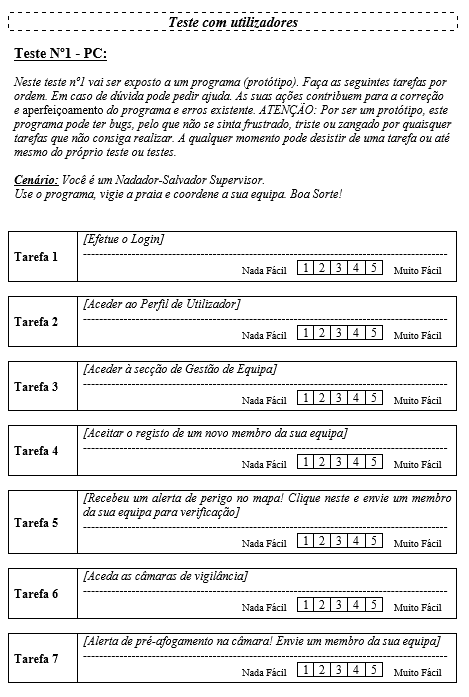
\includegraphics[width=14cm]{figs/UsabilityTest_Supervisor_1.png}
      \caption{Page 1 - Usability Tests to be carried out by Lifeguard Supervisors}
      \label{fig:UsabilityTest_Supervisor}
\end{figure}
\begin{figure}[H]
      \centering
      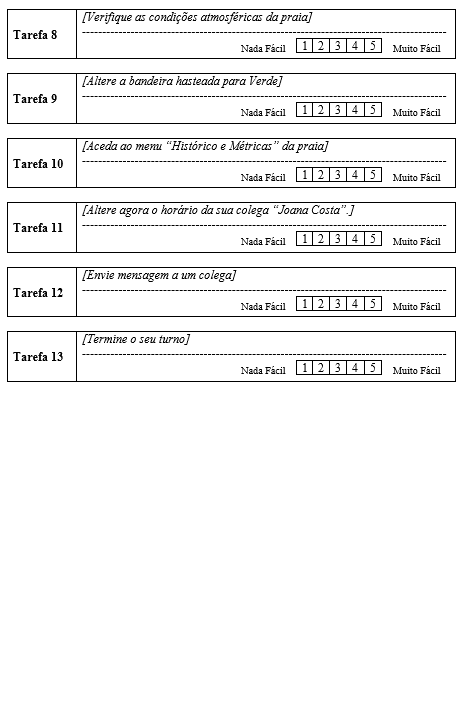
\includegraphics[width=14cm]{figs/UsabilityTest_Supervisor_2.png}
      \caption{Page 2 - Usability Tests to be carried out by Lifeguard Supervisors}
      \label{fig:UsabilityTest_Supervisor1}
\end{figure}

\subsection{Usability Tests: Regular Lifeguard}
\label{section:task_regular_lifeguard}

\begin{figure}[H]
      \centering
      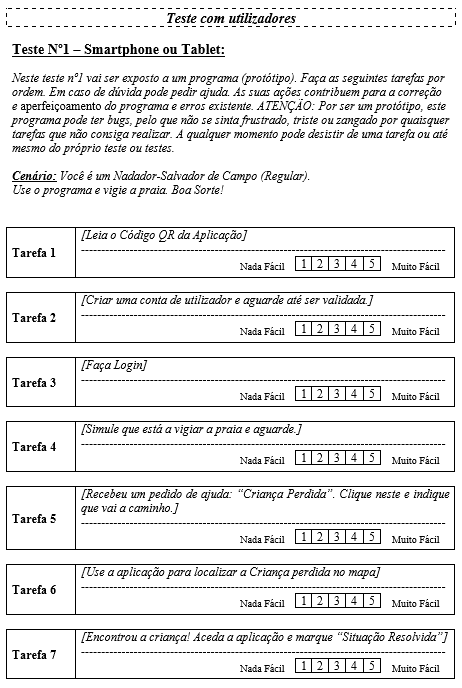
\includegraphics[width=14cm]{figs/UsabilityTest_Regular_1.png}
      \caption{Page 1 - Usability Tests to be carried out by Regular Lifeguards}
      \label{fig:UsabilityTest_Regular_1}
\end{figure}
\begin{figure}[H]
      \centering
      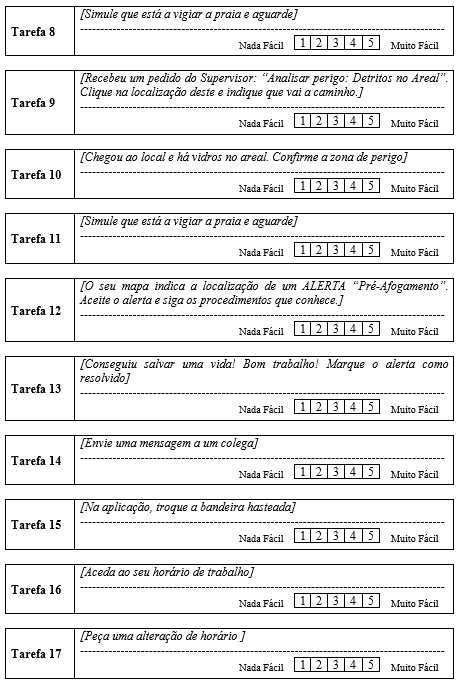
\includegraphics[width=14cm]{figs/UsabilityTest_Regular_2.png}
      \caption{Page 2 - Usability Tests to be carried out by Regular Lifeguards}
      \label{fig:UsabilityTest_Regular_2}
\end{figure}

\subsection{Usability Tests: Beachgoer \& Beach Business Owner}
\label{section:task_regular_lifeguard}
\texttt{Note: Since a Beach Business Owner can also be a Beachgoer, and a Beachgoer may take on the role of a Business Owner, the project includes a single task analysis test that applies to both user types.}

\begin{figure}[H]
      \centering
      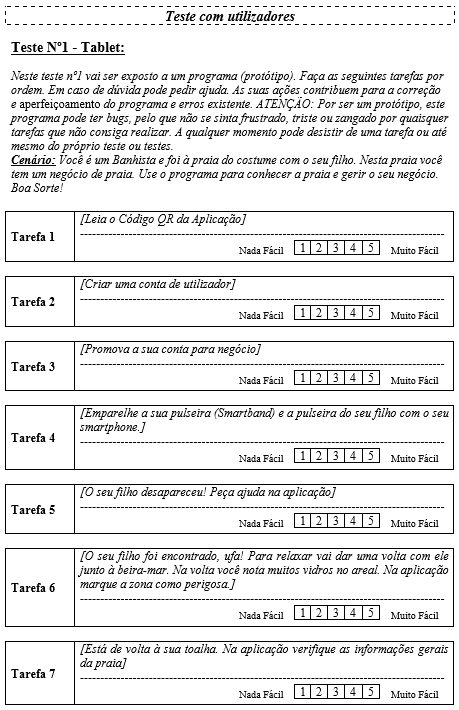
\includegraphics[width=14cm]{figs/UsabilityTest_Beachgoers_1.png}
      \caption{Page 1 - Usability Tests to be carried out by Beachgoers and Beach Business Owners}
      \label{fig:UsabilityTest_Beachgoers_1}
\end{figure}
\begin{figure}[H]
      \centering
      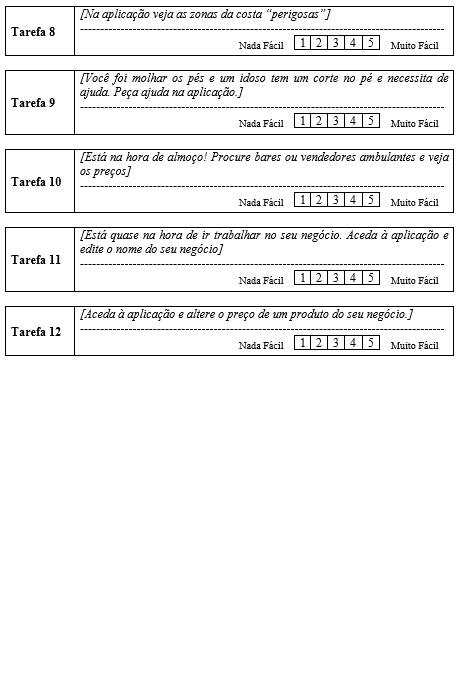
\includegraphics[width=14cm]{figs/UsabilityTest_Beachgoers_2.png}
      \caption{Page 2 - Usability Tests to be carried out by Beachgoers and Beach Business}
      \label{fig:UsabilityTest_Beachgoers_2}
\end{figure}

